% !TeX spellcheck = <none>
\documentclass[a4paper,11pt,twoside]{book}
\usepackage{amsmath}
\usepackage{graphicx}
\usepackage{siunitx}
\usepackage{setspace}
\usepackage[english,italian]{babel}
\usepackage[utf8]{inputenc}
\usepackage{ fancyhdr }

\makeatletter 
\renewcommand{\frontmatter}{% 
	\cleardoublepage\@mainmatterfalse 
	\pagenumbering{smallRoman}} 
\DeclareRobustCommand{\@smrc}[1]{% 
	\begingroup$\m@th$\fontsize{\sf@size}{\sf@size}\selectfont#1\endgroup} 
\def\smallRoman#1{\expandafter\@smallRoman\csname c@#1\endcsname} 
\def\@smallRoman#1{\@smrc{\expandafter\@slowromansmallcap\romannumeral #1@}} 
\def\@slowromansmallcap#1{\ifx @#1% then terminate 
	\else 
	\if i#1I\else 
	\if v#1V\else 
	\if x#1X\else 
	\if l#1L\else 
	\if c#1C\else 
	\if d#1D\else 
	\if m#1M\else 
	#1\fi\fi\fi\fi\fi\fi\fi 
	\expandafter\@slowromansmallcap 
	\fi 
} 
\makeatother
\begin{document}

\thispagestyle{empty}
\begin{center}
	\begin{Huge}
		\textsc{Progetto ``model-based''\\
				del controllo di robot Lego\\
				in ambiente Simulink\\}
	\end{Huge}
\end{center}
\vfill
\begin{center}
	\includegraphics[scale=0.35]{logo_unige.png}
\end{center}
\vfill
\begin{center}
	{\LARGE Francesco Tornatore Luca Lazzaroni}
\end{center}

\begin{center}
	{\Large DITEN - Dipartimento di Ingegneria Navale, Elettrica,\\
	Elettronica e delle Telecomunicazioni}
\end{center}
\begin{center}
	{\Large Università degli Studi di Genova}	
\end{center}
\vfill
\begin{center}
	{\large Tesi di Laurea Triennale}
\end{center}
\begin{center}
	{\large 27 Ottobre 2017}
\end{center}

\vfill


\newpage\null\thispagestyle{empty}\newpage

\frontmatter
\thispagestyle{empty}
\null\vspace{\stretch {1}}
\begin{center}
	\section*{Ringraziamenti}
		Ringraziamo il professor Marco Baglietto che ci ha guidati in questo nostro primo `lavoro'
\end{center}
\vspace{\stretch {2}}\null
\newpage
\begin{flushright}
	\null\vspace{\stretch {1}}
	A chi ci paga gli studi e a chi ci aiuta a non abbandonarli,\\ a buon rendere...
	\vspace{\stretch {2}}\null
\end{flushright}

\tableofcontents
\listoffigures
\listoftables
\mainmatter
\chapter{Introduzione}
Nel seguente elaborato si affronta il problema della modellazione e conseguente controllo di un sistema fisico realizzato con dispositivo LEGO MINDSTORM EV3 e alcuni tra i principali sensori e attuatori disponibili per questo modello.
In particolare i componenti utilizzati oltre al Brick, un microcontrollore all'interno del quale vengono caricati i programmi da eseguire, sono un potente motore e un sensore di posizione angolare detto encoder.

La scelta di questa tesi è dovuta alla volontà di mettersi alla prova per la prima volta con un progetto completo che comprendesse tutte le fasi di realizzazione, dalla modellazione alla sintesi, di un sistema.\\

L'obiettivo principale è quello di applicare i fondamenti della Teoria dei Sistemi e dei Controlli Automatici per controllare e smorzare l'oscillazione di un pendolo su di un carrello con trazione motrice.\\
Va precisato però, che chiamandola Teoria dei Sistemi, in realtà si omette un termine importante: per essere più precisi si dovrebbe infatti parlare di Teoria dei Sistemi Dinamici, dove con il termine “sistemi dinamici” ci riferiamo genericamente a tutte quelle entità che evolvono nel tempo secondo leggi di causalità e che interagiscono con l’ambiente mediante un principio di causa–effetto. Con Controlli Automatici, invece, ci riferiamo alla scienza che si prefigge di modificare il comportamento del sistema da controllare, ovvero delle sue uscite, attraverso la manipolazione delle grandezze d'ingresso.\\

Come altro obiettivo, ma non per questo meno importante, c'è l'intento di fornire del materiale didattico da mostrare a studenti che si accingono ad affrontare argomenti come quelli trattati per la prima volta, in modo da rendere più interessante e pragmatica una materia che durante il corso degli studi vedranno quasi esclusivamente su carta, e magari suscitare in loro il desiderio di continuare il nostro percorso in una nuova tesi.\\ 

Proprio per tali motivi abbiamo deciso di non utilizzare l'ambiente di sviluppo proprietario della casa produttrice, il quale vela tutta la teoria dei sistemi dinamici e del controllo che si nasconde dietro al funzionamento della Tecnologia LEGO, per adottare un approccio più ingegneristico.\\
Per la modellazione, la simulazione e l'analisi del sistema si fa uso dell'ambiente di sviluppo Simulink, strettamente integrato con MATLAB, il quale fornisce una miriade di strumenti utili al progetto.

Grazie al suddetto ambiente si riesce a stabilire una connessione WI-FI(con l'ausilio dell'adattatore wireless USB Netgear WNA1100) oppure USB tra PC e robot con la quale il programma viene caricato ed in seguito eseguito in modalità autonoma o guidata, a seconda delle esigenze, tramite l'impostazione di alcuni parametri.\\

Nei seguenti capitoli, dopo un'attenta analisi della risposta al gradino, si procede con l'identificazione del modello del motore LEGO utilizzato per la locomozione.\\
Si prosegue scrivendo le equazioni fisiche del modello del pendolo su carrello, facendo alcune considerazioni su quelle che sono le approssimazioni fatte per semplificarlo.\\
Una volta individuati gli ingressi, le variabili di stato e le uscite di interesse, le equazioni di stato sono facilmente ricavabili.

Siccome la quasi totalità dei sistemi fisici è non lineare, la ricerca di soluzioni analitiche è molto difficile e a volte impossibile. È solitamente possibile trasformare un problema non lineare in un problema localmente lineare, cioè trovare un sistema lineare che approssimi, entro un certo raggio, il sistema non lineare originale.
Quindi si cercano i punti di equilibrio e infine si linearizzano le equazioni di stato attorno a tali punti.

Per ricostruire ora il sistema complessivo, bisogna esaminare la relazione tra l'uscita del primo, il motore, e l'ingresso del secondo, il carrello, così da aggiungere un sistema intermedio che trasformi e adatti il segnale tra i due blocchi principali.\\
Ricavata la funzione di trasferimento totale si analizza la stabilità con i sopracitati strumenti di MATLAB e si ricercano  i possibili regolatori adatti a velocizzare la risposta del sistema agli stimoli in modo da ridurre il tempo di assestamento nella maniera desiderata.\\




\chapter{Modello del motore}
\section{Dalla potenza alla velocità angolare}

\begin{figure}[ht]
	\centering
	\includegraphics[width=\textwidth]{motoreSimulink.jpg}
	\caption{Schema a blocchi Motore}
	\label{motoreSimulink}
\end{figure}
Il LEGO MINDSTORM EV3 è dotato di un motore, l'EV3 Large Servo Motor, la cui velocità angolare, misurata in $rad/s$, è stata assunta come uscita del sistema.\\
I valori di ingresso possibili sono invece compresi tra -100 e +100, dove +100 indica la massima potenza erogabile, mentre -100 idem, ma con verso di rotazione opposto.\\
Al fine di modellare nel modo più preciso possibile abbiamo applicato a tale motore un albero dotato di pesi posti a una certa distanza da quest'ultimo in modo tale da incrementare il momento d'inerzia $I$ e, di conseguenza, diminuire l'accelerazione angolare massima $\alpha$ in accordo con la seconda legge di Newton (in forma angolare) $\tau = I\alpha$, dove $\tau$ è il momento della forza o, più semplicemente, la coppia massima erogata: valore caratteristico del motore.
\newpage
\begin{figure}[ht]
	\centering
	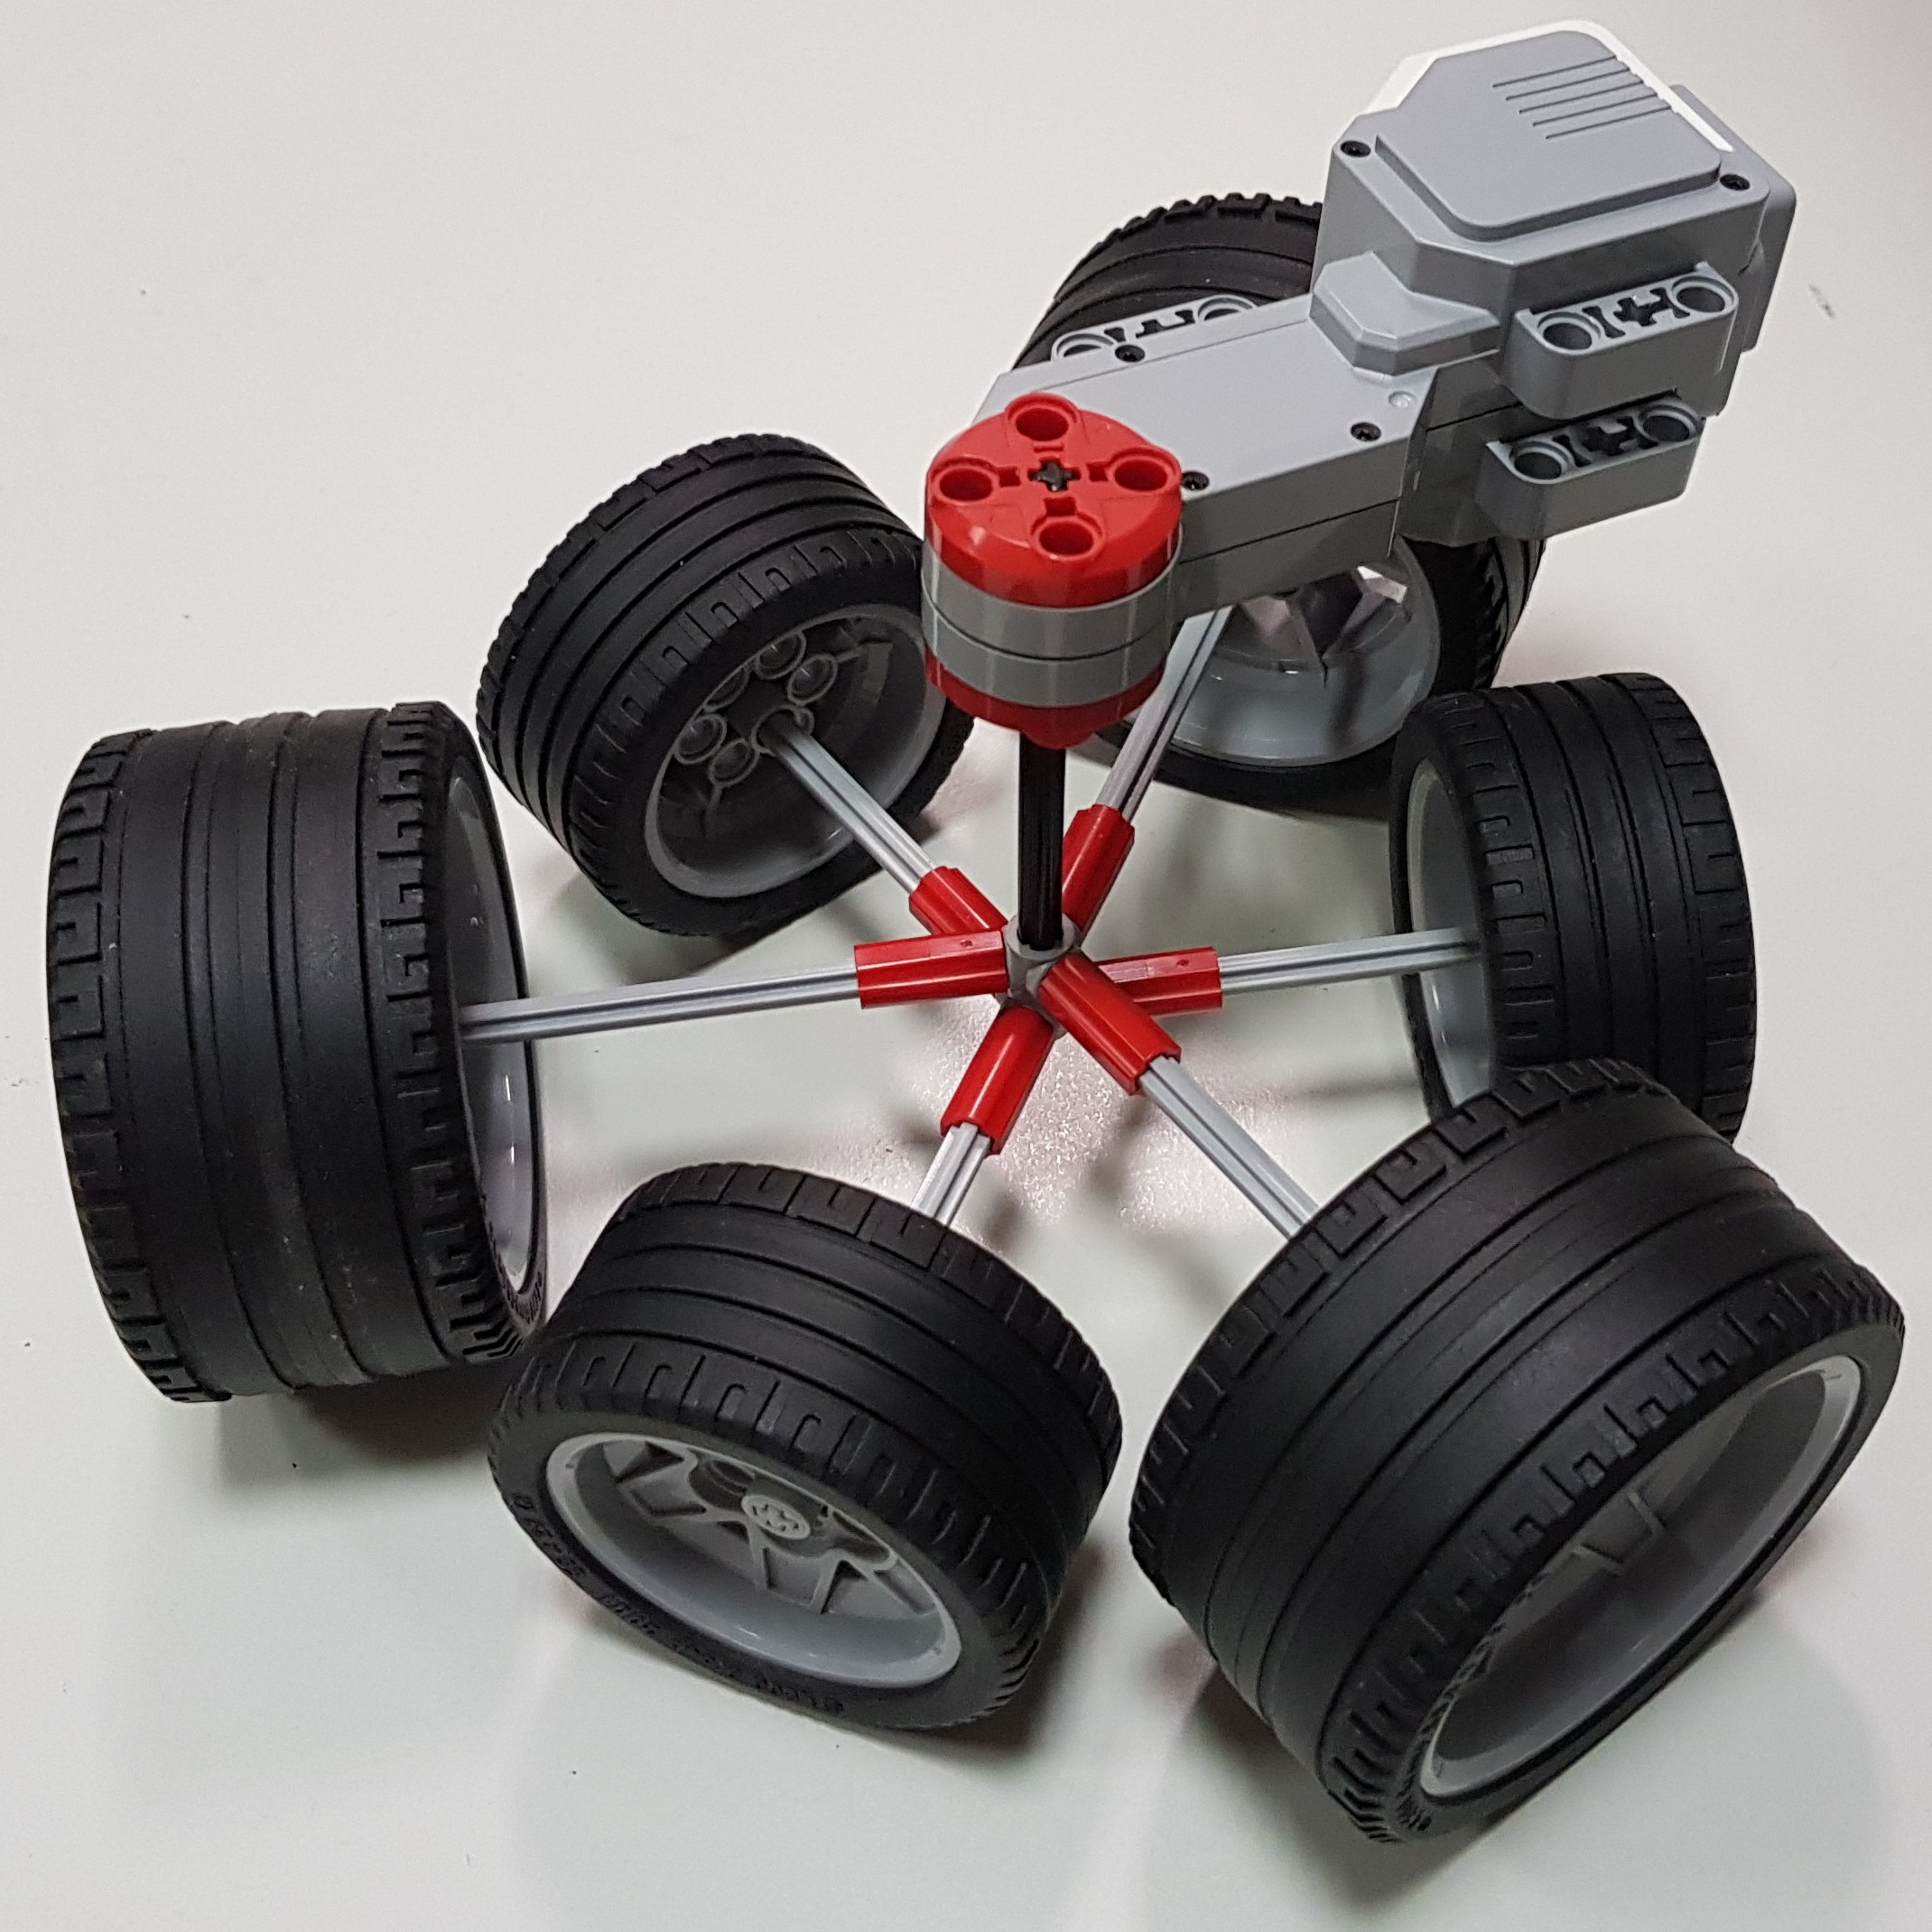
\includegraphics[width=\textwidth]{megainerzia.png}
	\caption{Albero per aumentare Inerzia del motore}
	\label{megainerzia}
\end{figure}
In questo modo il tempo di assestamento $t_a$ del sistema, direttamente proporzionale a $\alpha$, è sensibilmente più lungo ed è dunque più semplice trovare una funzione di trasferimento assimilabile a quella dell'EV3 Large Servo Motor.\\
All'interno del motore è inoltre presente un'encoder che permette di misurare, in gradi, la posizione angolare dello stesso.
Di conseguenza, al fine di ottenere la velocità angolare $\omega$ è stato applicato in cascata un derivatore, ma anche un filtro passa basso con frequenza di taglio $\omega_c=25\;Hz$, necessario per attenuare le alte frequenze del sistema, al fine di ottenere una funzione in uscita meno spezzata possibile e, di conseguenza, più facilmente identificabile.\\
Al fine di ridurre il più possibile l'errore è stato scelto come tempo di campionamento dell'encoder il valore minimo supportato: 0.001 $s$.\\
Il risultato che si ottiene utilizzando come ingresso una funzione gradino con valore finale pari a 50 è mostrato nella figura \ref{motore50StepCamp1000}.
\begin{figure}[ht]
	\centering
	\includegraphics[width=\textwidth]{motore50StepCamp1000.jpg}
	\caption{Risposta al gradino con $\omega_c=25\;Hz$}
	\label{motore50StepCamp1000}
\end{figure}
\\Scegliendo invece una frequenza di taglio del filtro passa basso $\omega_c = 100Hz$ l'uscita del sistema diventa:
\begin{figure}[ht]
	\centering
	\includegraphics[width=\textwidth]{motore50StepCamp1000Polo100.jpg}
	\caption{Risposta al gradino con $\omega_c=100\;Hz$ }
	\label{motore50StepCamp1000Polo100}
\end{figure}
\\Si può notare come la frequenza di taglio sia troppo elevata non attenuando abbastanza le alte frequenze e rendendo così impossibile una stima della funzione di trasferimento.\\
Prendendo quindi in esame il primo dei due grafici si può stimare una costante di tempo $\tau$ (tempo che impiega la funzione a raggiungere il 63\% del valore di regime) del sistema pari a circa 0.15 $s$ e guadagno statico 10.4.\\\\
La funzione di trasferimento che ne consegue è dunque:
\\
$$
T_{motore}(s)=\displaystyle\frac{10.4}{0.15s+1}
$$
\\
Di seguito un confronto tra $T_{motore}(s)$ e la funzione di trasferimento reale del motore.
\begin{figure}[ht]
	\centering
	\includegraphics[width=\textwidth]{modMotorvsReale.jpg}
	\caption{Risposta al gradino del Motore reale e del suo modello}
	\label{modMotorvsReale}
\end{figure}

\section{Dalla velocità angolare alla coppia}
È necessario ora ottenere la coppia generata dal motore in funzione del tempo al fine di utilizzarla come ingresso per la funzione di trasferimento del pendolo che sarà trattata in modo approfondito nel prossimo capitolo.\\
La formula utilizzata per calcolare tale coppia è la seguente:
$$
\tau=K\omega+I\alpha
$$
Dove il primo termine dell'equazione indica appunto la coppia, mentre i restanti due sono rispettivamente lo smorzamento viscoso e il momento torcente.
Più nello specifico $K$ rappresenta il coefficiente di smorzamento viscoso misurato in $Nm\,s/rad$, $\omega$ la velocità angolare, $I$ il momento d'inerzia del sistema e $\alpha$ l'accelerazione angolare.\\
Calcoliamo innanzi tutto $I$: 
$$
I=3M_Rd_R^2+3M_rd_r^2+3I_a+3I_A+\displaystyle\frac{m_ar^2}{2}
$$
Il primi due termini indicano i momenti d'inerzia delle sei ruote (assunte come masse uniformi per semplicità), il terzo e il quarto quelli delle sei aste che collegano le ruote all'albero, mentre l'ultimo termine rappresenta il momento d'inerzia dell'albero (asta centrale).\\
Per calcolare $I$ delle sei aste utilizziamo il teorema di Huygens-Steiner, o degli assi paralleli:
$$
I=I_{cdm}+m_{asta}d^2
$$
Dove $d$ è la distanza tra l'asse passante per il centro di massa e quello parallelo di rotazione (rispetto al quale calcoliamo il momento).\\
$$
I_{asta}=\displaystyle\frac{1}{12}m_{asta}l^2+m_{asta}(\displaystyle\frac{l}{2})^2=\displaystyle\frac{1}{3}m_{asta}l^2
$$
Inserendo ora i parametri calcolati sperimentalmente e riportati nella tabella sottostante, si ricava un momento d'inerzia $I$ pari a 0.001364 $Kg\,m^2$.\\\\
\begin{tabular}{|l|l|l|l|}
	\hline
	\textbf{Sigla} & \textbf{Valore} & \textbf{U.d.m.} & \textbf{Parametro}\\
	\hline
	$M_R$ & 0.0395 & $kg$ & massa ruota grande\\
	\hline
	$M_r$ & 0.023 & $kg$ & massa ruota piccola\\
	\hline
	$m_a$ & 0.0015 & $kg$ & massa asta corta\\	
	\hline
	$m_A$ & 0.002 & $kg$ & massa asta lunga\\	
	\hline
	$l_a$ & 0.068 & $m$ & lunghezza asta corta\\
	\hline
	$r$ & 0.002 & $m$ & raggio asta\\
	\hline
	$l_A$ & 0.091 & $m$ & lunghezza asta lunga\\
	\hline
	$d_r$ & 0.061 & $m$ & distanza ruota piccola - asse di rotazione\\
	\hline
	$d_R$ & 0.085 & $m$  & distanza ruota grande - asse di rotazione\\
	\hline
\end{tabular}\\\\\\
Essendo $\tau=K\omega+I\alpha$ possiamo disegnare tramite Simulink il diagramma a blocchi rappresentato in figura \ref{modMotoreTorque}:
\begin{figure}[ht]
	\centering
	\includegraphics[width=\textwidth]{modMotoreTorque.jpg}
	\caption{Modello completo del Motore}
	\label{modMotoreTorque}
\end{figure}
\\L'uscita del sistema è proprio la coppia $\tau$ desiderata.\\
Si può notare come nel blocco inferiore siano stati aggiunti il derivatore e il filtro passa basso.\\
Il primo è necessario dal momento che l'accelerazione angolare $\alpha$ è proprio la derivata della velocità angolare $\omega$.\\
Per quanto riguarda il filtro, invece, è stato aggiunto (scegliendo appositamente una frequenza di taglio abbastanza alta da non alterare la dinamica del sistema) siccome un derivatore puro è fisicamente irrealizzabile (funzione impropria).\\
Inoltre si è resa necessaria anche l'aggiunta di un blocco di saturazione dell'ingresso dal momento che, come già reso noto in precedenza, l'EV3 Large Servo Motor accetta valori compresi tra -100 e +100.\\
In ultimo il valore di K è stato invece ricavato sperimentalmente avendo nota la coppia a regime, caratteristica dell'EV3 Large Servo Motor e pari a 0.2 $Nm$.\\
Come si mostrato in figura \ref{torque02} un valore di K pari a 0.000192 $Nm\,s/rad$ consente di rispettare appieno tale specifica.
\begin{figure}[ht]
	\centering
	\includegraphics[width=\textwidth]{torque02.jpg}
	\caption{Risposta al gradino del modello completo}
	\label{torque02}
\end{figure}
\chapter{Pendolo su carrello}\label{PendCarrello}
\section{Modello e relative equazioni}

\begin{figure}[ht]
	\centering
	\includegraphics[width=\textwidth]{pendolo.png}\\
	\caption{Modello del pendolo su carrello}
	\label{pendolo}
\end{figure}
\textbf{Bilanciamento forze sull'asta}\\
Asse X:
\begin{equation}\notag
m\ddot{x}_m=H
\end{equation}
Asse Y:
\begin{equation}\notag
m\ddot{y}_m=V-mg
\end{equation}
Dove $H$ e $V$ sono le reazioni vincolari (orizzontale e verticale) a cui e sottoposta la massa $m$ per il fatto di essere bloccata all'estremità dell'asta.\\ 
Essendo:\\
\begin{equation}\notag
x_m = x_M+l_a\sin(\theta) \quad \Rightarrow \quad \ddot{x}_m=\ddot{x}_M-l_a\sin(\theta)\dot{\theta}^2+l_a\cos(\theta)\ddot{\theta}
\end{equation}
\begin{equation}\notag
y_m=y_M-l_a\cos(\theta) \quad \Rightarrow \quad \ddot{y}_m=l_a\sin(\theta)\ddot{\theta}+l_a\cos(\theta)\dot{\theta}^2
\end{equation}
Si ottiene:
\begin{equation}\label{Hv}
H=m\ddot{x}_M-ml_a\sin(\theta)\dot{\theta}^2+ml_a\cos(\theta)\ddot{\theta}
\end{equation}
\begin{equation}\label{Vv}
V=mg+ml_a\cos(\theta)\dot{\theta}^2+ml_a\sin(\theta)\ddot{\theta}
\end{equation}
\textbf{Bilanciamento forze sul carrello}
\begin{equation}\notag
M\ddot{x}_M=u-H
\end{equation}
sostituendo la \ref{Hv} si ha:
$$
M\ddot{x}_M=u-m\ddot{x}_M+ml_a\sin(\theta)\dot{\theta}^2-ml_a\cos(\theta)\ddot{\theta}
$$
\begin{equation}\label{FCarr}
(M+m)\ddot{x}_M+ml_a\cos(\theta)\ddot{\theta}=u+ml_a\dot{\theta}^2\sin(\theta)
\end{equation} 
\textbf{Bilanciamento momenti del sistema asta-massa}
\begin{equation}
I_m\ddot{\theta}=l_aV\sin(\theta)+l_aH\cos(\theta)
\end{equation}
sostituendo la \ref{Hv} e la \ref{Vv}:
$$
I_m\ddot{\theta}=l_a\sin(\theta)[mg+ml_a\cos(\theta)\dot{\theta}^2+ml_a\sin(\theta)\ddot{\theta}]+$$$$+l_a\cos(\theta)[m\ddot{x}_M-ml_a\sin(\theta)\dot{\theta}^2+ml_a\cos(\theta)\ddot{\theta}]=
$$
$$
=mgl_a\sin(\theta)+ml_a^2\sin(\theta)\cos(\theta)\dot{\theta}^2+ml_a^2\sin^2(\theta)\ddot{\theta}+ml_a\ddot{x}_M\cos(\theta)+$$$$-ml_a^2\cos(\theta)\sin(\theta)\dot{\theta}^2
+ml_a^2\cos^2(\theta)\ddot{\theta}=$$
$$=mgl_a\sin(\theta)+ml_a^2\ddot{\theta}+ml_a\ddot{x}_M\cos(\theta) =
$$
\begin{equation} \label{momInThetaP}
=ml_a(g\sin(\theta)+l_a\ddot{\theta}+\ddot{x}_M\cos(\theta))
\end{equation}
Essendo il momento d'inerzia dell'asta $$
I_m=\displaystyle\frac{1}{12}m_al_a^2+m_a(\displaystyle\frac{l}{2})^2=\displaystyle\frac{1}{3}m_al_a^2=0.000045\quad kg\cdot m^2$$molto inferiore rispetto a quello della massa $m$ attaccata al pendolo, $$
I_m=ml_a^2=0.00041\quad kg\cdot m^2$$ possiamo per semplicità trascurarlo, per cui poniamo $I_m=0$.\\
Il sistema che deriva dalla \ref{FCarr} e dalla \ref{momInThetaP} è dunque il seguente:
\\\\
$\begin{cases}
$$(M+m)\ddot{x}_M+ml_a\cos(\theta)\ddot{\theta}=u+ml_a\dot{\theta}^2\sin(\theta)$$ \\
$$g\sin(\theta)+l_a\ddot{\theta}+\ddot{x}_M\cos(\theta)=0$$\\
\end{cases}
$
\\\\
Dalla prima equazione del sistema 
$$
(M+m)(\frac{-g\sin(\theta)-l_a\ddot{\theta}}{\cos(\theta)})+ml_a\cos(\theta)\ddot{\theta}=u+ml_a\dot{\theta}^2\sin(\theta)
$$
$$
\ddot{\theta}(ml_a\cos(\theta)-\frac{l_a(M+m)}{\cos(\theta)}=u+ml_a\dot{\theta}^2\sin(\theta)+\frac{g\sin(\theta)(M+m)}{\cos(\theta)}
$$
$$
\ddot{\theta}=\frac{[u+ml_a\dot{\theta}^2\sin(\theta)+\displaystyle\frac{g\sin(\theta)(M+m)}{\cos(\theta)}]\cos(\theta)}{ml_a\cos^2(\theta)-l_a(M+m)} \Rightarrow$$\\
\begin{equation}\label{theta2punti}
\ddot{\theta}=\frac{u\cos(\theta)+ml_a\dot{\theta}^2\sin(\theta)\cos(\theta)+g\sin(\theta)(M+m)}{-l_a(m\sin^2(\theta)+M)}
\end{equation}\\
Dalla seconda equazione del sistema
$$
\ddot{x}_M=\frac{-g\sin(\theta)-l_a\ddot{\theta}}{\cos(\theta)}
$$
e sostituendo ora la \ref{theta2punti}  
$$
\ddot{x}_M=\frac{-g\sin(\theta)-\displaystyle\frac{ul_a\cos(\theta)+ml^2_a\dot{\theta}^2\sin(\theta)\cos(\theta)+gl_a\sin(\theta)(M+m)}{-l_a(m\sin^2(\theta)+M)}}{\cos(\theta)}=
$$
$$
=\frac{g\sin(\theta)[-l_a(m\sin^2(\theta)+M)]+ul_a\cos(\theta)+ml^2_a\dot{\theta}^2\sin(\theta)\cos(\theta)+gl_a\sin(\theta)(M+m)}{l_a\cos(\theta)(m\sin^2(\theta)+M)}=
$$
$$
=\frac{-gm\sin^3(\theta)-gM\sin(\theta)+u\cos(\theta)+ml_a\dot{\theta}^2\sin(\theta)\cos(\theta)+gM\sin(\theta)+gm\sin(\theta)}{\cos(\theta)(m\sin^2(\theta)+M)}
$$
$$
=\frac{u+ml_a\dot{\theta}^2\sin(\theta)+gm\cos(\theta)\sin(\theta)}{m\sin^2(\theta)+M}
$$\\
Assegniamo le variabili di stato e definiamo le uscite desiderate:\\\\
$\begin{cases}
$$x_1 \stackrel{\Delta}{=} x_M$$ \\
$$x_2\stackrel{\Delta}{=}\dot{x}_M$$\\
$$x_3\stackrel{\Delta}{=}\theta$$\\
$$x_4\stackrel{\Delta}{=}\dot{\theta}$$\\
$$y_1\stackrel{\Delta}{=}x_M$$ \\
$$y_2\stackrel{\Delta}{=}\theta$$\\
\end{cases}
$\\\\\\
Sostituendo queste ultime nelle equazioni appena ricavate si ottengono le equazioni:
\\\\\\
$\underline{\dot{x}}=\displaystyle\frac{d}{d t}
\begin{bmatrix}
x_M\\\\
\dot{x}_M\\\\
\theta\\\\
\dot{\theta}\\\\
\end{bmatrix}
=
\begin{bmatrix}
x_2\\\\
\displaystyle\frac{u+ml_ax_4^2\sin(x_3)+gm\cos(x_3)\sin(x_3)}{m\sin^2(x_3)+M}\\\\
x_4\\\\
-\displaystyle\frac{u\cos(x_3)+ml_ax_4^2\sin(x_3)\cos(x_3)+g(M+m)\sin(x_3)}{l_a(m\sin^2(x_3)+M)}\\\\
\end{bmatrix}
$
\\\\\\
\section{Linearizzazione del modello}\label{LinMod}
\textbf{Punti di equilibrio del sistema} \\
Per la ricerca dei punti di equilibrio poniamo $\underline{f}(\underline{x},u)=\underline{0}$\quad(dove $\underline{\dot{x}}=\underline{f}(\underline{x},u$)):\\\\
$\begin{cases}
$$x_2=0$$ \\
$$\displaystyle\frac{u+ml_ax_4^2\sin(x_3)+gm\cos(x_3)\sin(x_3)}{m\sin^2(x_3)+M}=0$$\\
$$x_4=0$$\\
$$\displaystyle\frac{u\cos(x_3)+ml_ax_4^2\sin(x_3)\cos(x_3)+g(M+m)\sin(x_3)}{l_a(m\sin^2(x_3)+M)}=0$$
\end{cases}
$\\\\\\
Dal precedente sistema si capisce che punti di equilibrio del pendolo su carrello sono due, uno instabile per \\
$\begin{cases}
$$x_1=\forall$$ \\
$$x_2=0$$\\
$$x_3=\pm\pi$$\\
$$x_4=0$$\\
$$u=0$$
\end{cases}$\\
ovvero quando il pendolo è rivolto verso l'alto (pendolo inverso), l'altro, stabile, per\\
$\begin{cases}
$$x_1=\forall$$ \\
$$x_2=0$$\\
$$x_3=0$$\\
$$x_4=0$$\\
$$u=0$$
\end{cases}$\\
quando il pendolo è rivolto verso il basso (pendolo "normale").
Siccome il punto di equilibrio non dipende dalla posizione del carrello possiamo per semplicità scegliere $x_1=0$.\\\\
\textbf{Linearizzazione del sistema attorno al punto di equilibrio}\\
Vogliamo ora linearizzare le precedenti equazioni di stato attorno al punto di equilibrio $\underline{\tilde{x}}=\underline{0}$, $\tilde{u}=0$ trovato: \\\\
$\displaystyle\frac{\partial{f_1}}{\partial{\underline{x}}}(\underline x,u)=
\begin{bmatrix}
0&1&0&0
\end{bmatrix}$\qquad
$\displaystyle\frac{\partial{f_1}}{\partial{u}}(\underline{x},u)=0$\\\\\\
$\displaystyle\frac{\partial{f_2}}{\partial{x_1}}(\underline{x},u)=0$\qquad
$\displaystyle\frac{\partial{f_2}}{\partial{x_2}}(\underline{x},u)=0$\\
$\displaystyle\frac{\partial{f_2}}{\partial{x_3}}(\underline{x},u)=\displaystyle\frac{[ml_ax_4^2\cos(x_3)+mg(\cos^2(x_3)-\sin^2(x_3))](M+m\sin^2(x_3))}{(M+m\sin^2(x_3))^2}$\\
$-\displaystyle\frac{[u+ml_ax_4^2\sin(x_3)+mg\sin(x_3)\cos(x_3)](2\sin(x_3)\cos(x_3))}{(M+m\sin^2(x_3))^2}\bigg|_{\underline{\tilde{x}},\tilde{u}}=\displaystyle\frac{mg}{M}$\\ $\displaystyle\frac{\partial{f_2}}{\partial{x_4}}(\underline{x},u)=\displaystyle\frac{2ml_a\sin(x_3)x_4}{M+m\sin^2(x_3)}\bigg|_{\underline{\tilde{x}},\tilde{u}}=0$\quad$\displaystyle\frac{\partial{f_2}}{\partial{u}}(\underline{x},u)=\displaystyle\frac{1}{M+m\sin^2(x_3)}\bigg|_{\underline{\tilde{x}},\tilde{u}}=\displaystyle\frac{1}{M}$\\\\\\
$\displaystyle\frac{\partial{f_3}}{\partial{\underline{x}}}(\underline x,u)=
\begin{bmatrix}
0&0&0&1
\end{bmatrix}$\qquad$\displaystyle\frac{\partial{f_3}}{\partial{u}}(\underline{x},u)=0$\\\\\\
$\displaystyle\frac{\partial{f_4}}{\partial{x_1}}(\underline{x},u)=0$\qquad
$\displaystyle\frac{\partial{f_4}}{\partial{x_2}}(\underline{x},u)=0$\\
$\displaystyle\frac{\partial{f_4}}{\partial{x_3}}(\underline{x},u)=\displaystyle\frac{[u\sin(x_3)-ml_ax_4^2(\cos^2(x_3)-\sin^2(x_3))-g\cos(x_3)(M+m)][l_a(m\sin^2(x_3)+M)]}{l_a^2(m\sin^2(x_3)+M)^2}+$ $-\displaystyle\frac{[-u\cos(x_3)-ml_ax^2_4\sin(x_3)\cos(x_3)-g\sin(x_3)(m+M)][2ml_a\sin(x_3)\cos(x_3)]}{l_a^2(m\sin^2(x_3)+M)^2}\bigg|_{\underline{\tilde{x}},\tilde{u}}=$
$=-\displaystyle\frac{(M+m)g}{Ml}$\qquad$\displaystyle\frac{\partial{f_4}}{\partial{x_4}}(\underline{x},u)=\displaystyle\frac{-2ml_ax_4\sin(x_3)\cos(x_3)}{l_a(m\sin^2(x_3)+M)}\bigg|_{\underline{\tilde{x}},\tilde{u}}=0$\\$\displaystyle\frac{\partial{f_4}}{\partial{u}}(\underline{x},u)=\displaystyle\frac{-\cos(x_3)}{l_a(m\sin^2(x_3)+M)}\bigg|_{\underline{\tilde{x}},\tilde{u}}=-\displaystyle\frac{1}{ml_a}$\\\\\\
Le equazioni linearizzate sono dunque:\\\\
$\underline{\delta\dot{x}}=
\begin{bmatrix}
0&1&0&0\\
0&0&\displaystyle\frac{mg}{M}&0\\
0&0&0&1\\
0&0&-\displaystyle\frac{(M+m)g}{Ml_a}&0
\end{bmatrix}
\underline{\delta x}+
\begin{bmatrix}
0\\
\displaystyle\frac{1}{M}\\
0\\
-\displaystyle\frac{1}{Ml_a}\\
\end{bmatrix}
\underline{\delta u}
$\\\\
$\underline{\delta y}=
\begin{bmatrix}
1&0&0&0\\
0&0&1&0
\end{bmatrix}
\underline{\delta x}
$\\\\\\
Calcolando ora la funzione di trasferimento $T(s)$ tra l'ingresso $u$ (forza esercitata sul carrello,
avanti/indietro) e l'uscita $y_2$(angolo $\theta$ del pendolo rispetto alla verticale) si ottiene:\\\\
$T_{y_2,u}(s)=C(sI-A)^{-1}B=
\begin{bmatrix}
0&0&1&0
\end{bmatrix}
\begin{bmatrix}
*&*&*&*\\
*&*&*&*\\
*&0&*&\displaystyle\frac{1}{s^2+\frac{(M+m)g}{Ml_a}}\\
*&*&*&*
\end{bmatrix}
\begin{bmatrix}
0\\
\displaystyle\frac{1}{M}\\
0\\
-\displaystyle\frac{1}{Ml_a}\\
\end{bmatrix} = \\
=-\displaystyle\frac{1}{Ml_as^2+(M+m)g}
$\\\\\\
Inserendo ora i parametri del modello fisico del pendolo su  carrello realizzato con l'ausilio del Lego MINDSTORM EV3 si può procedere all'identificazione della funzione di trasferimento.
\begin{table}[ht]
	\begin{tabular}{|l|l|l|l|}
		\hline
		\textbf{Sigla} & \textbf{Valore} & \textbf{U.d.m.} & \textbf{Parametro}\\
		\hline
		$M$ & 0.7535 & $kg$ & massa carrello\\
		\hline
		$m$ & 0.016 & $kg$ & massa all'estremità del pendolo\\
		\hline
		$g$ & 9.81 & $m/s^2$ & accelerazione di gravità\\
		\hline
		$l_a$ & 0.166 & $m$ & lunghezza asta del pendolo\\
		\hline
		$r$ & 0.034 & $m$ & raggio ruote motrici\\
		\hline
	
	\end{tabular}	
\caption{Parametri del sistema Carrello-Pendolo}
\label{carrPend}
\end{table}
\\Data la tabella \ref{carrPend} si ha:
$$T_{y_2,u}(s)=-\displaystyle\frac{1}{0.125s^2+7.541}$$
\newpage
\section{Stabilizzazione del pendolo}
Il pendolo di per sè è un sistema già stabile, lo scopo della realizzazione su carrello consiste nello smorzarne l'oscillazione riducendo la costante di tempo del sistema grazie all'impiego di due ruote motrici.\\
In figura \ref{pendoloFisico} realizzazione del pendolo su carrello utilizzando un motore EV3 Large Servo Motor come trazione e un encoder GlideWheel-M per misurare l'angolo del pendolo 
\begin{figure}[ht]
	\centering
	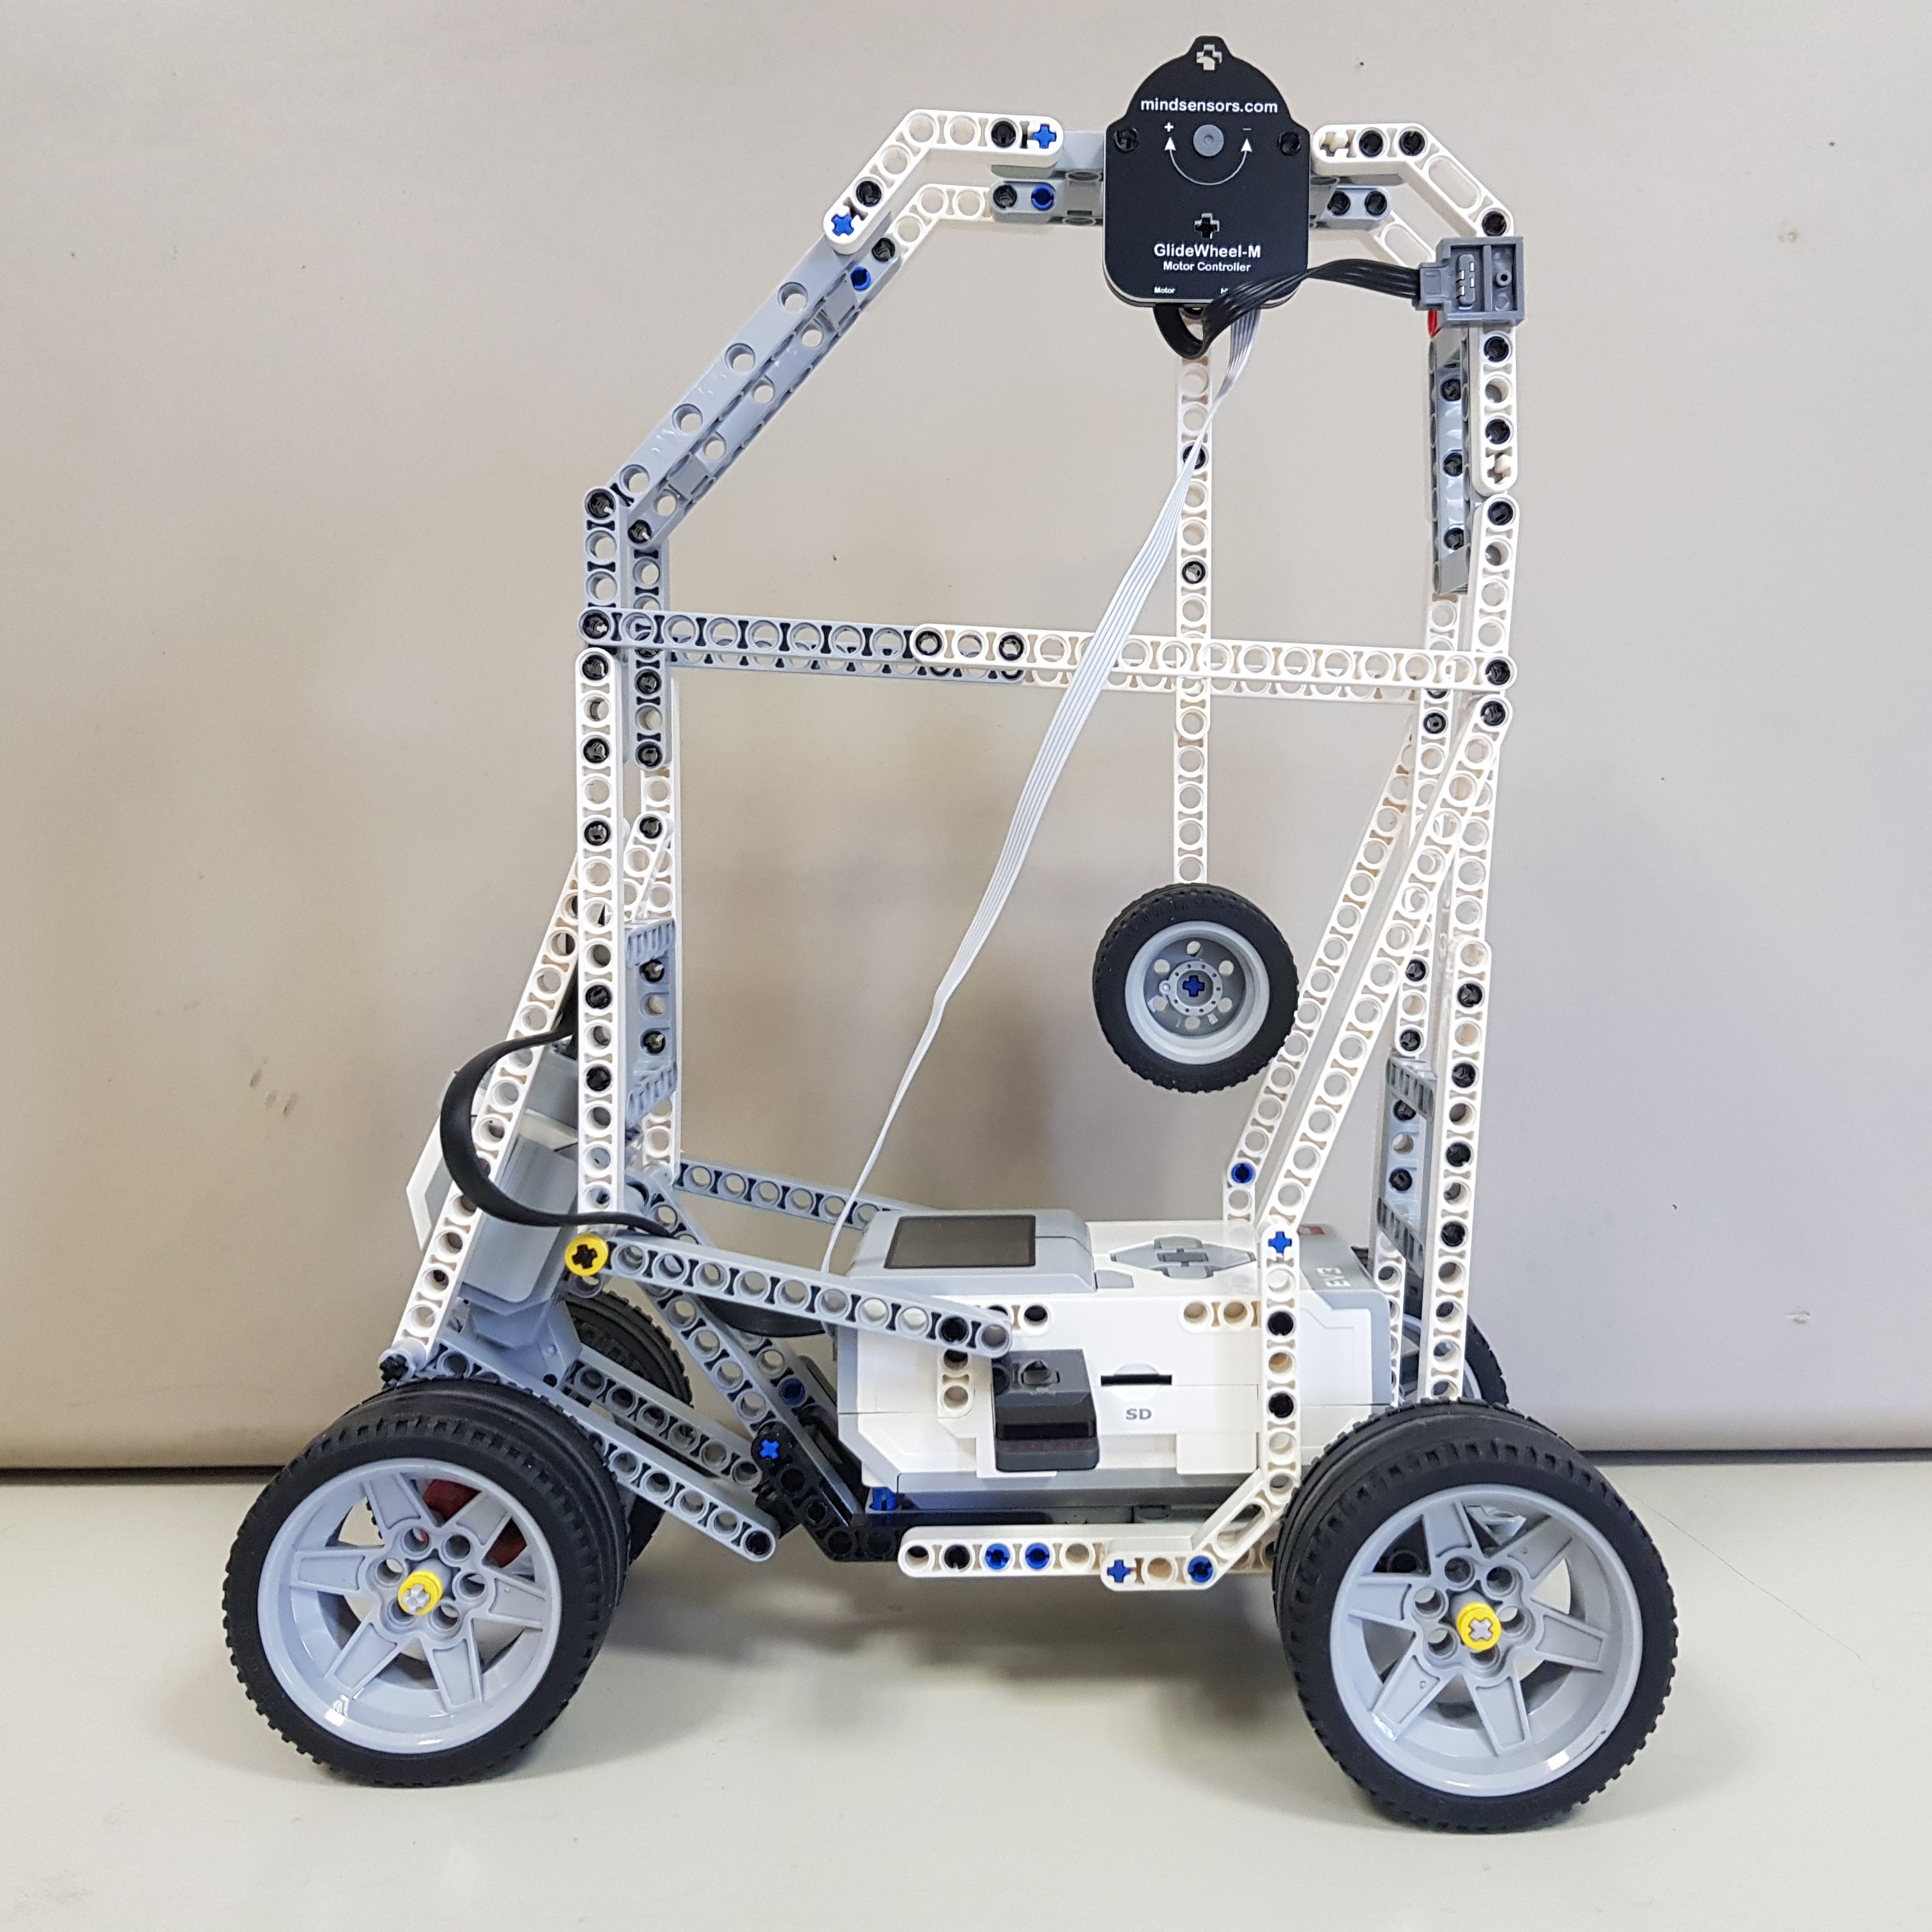
\includegraphics[scale=0.08]{pendoloFisico.jpg}\\
	\caption{Realizzazione fisica del pendolo su carrello}
	\label{pendoloFisico}
\end{figure} 
rispetto alla verticale.\\
Da specifiche quest'ultimo può raggiungere un tempo di campionamento minimo di 0.001s (così come il motore) ma a tale valore non riesce sempre a campionare in modo corretto, perciò abbiamo deciso di aumentarlo in modo da non perdere nessuna variazione anche alla massima velocità angolare raggiunta dal pendolo durante l'oscillazione libera tra $[\ang{-31},\ang{+31}]$ (intervallo entro il quale il pendolo è vincolato per costruzione).
\begin{figure}[ht]
	\centering
	\includegraphics[width=\textwidth]{SlewRate.PNG}\\
	\caption{Massima velocità di oscillazione libera}
	\label{slewRate}
\end{figure}
Da tale esperimento è risultato che durante la prima oscillazione (in figura \ref{slewRate}), il pendolo, raggiunge per $\theta=\ang{0}$ la velocità $\omega=250\deg/s$ (calcolata con un semplice rapporto incrementale) per cui il tempo di campionamento ottimale sarebbe stato $t_c=\displaystyle\frac{1}{250}=0.004s$.
Sfruttando il modello del motore LEGO da noi ricavato si può quindi ricavare la funzione di Trasferimento del sistema complessivo (avente come ingresso la potenza richiesta al motore e come uscita la posizione angolare del pendolo).\\
Siccome in uscita al modello del motore abbiamo la coppia erogata dallo stesso, per poterlo mettere in serie al modello del pendolo su carrello (il quale come ingresso riceve una spinta sotto forma di forza) occorre adattare il collegamento I/O. Poiché si assume un puro moto di rotolamento delle ruote del carrello si tratta di trovare il giusto coefficiente $C$ di proporzionalità tra coppia e spinta.
\begin{figure}[ht]
	\centering
	\includegraphics[scale=0.4]{braccioForza.PNG}
	\caption{Momento della forza}
	\label{braccioForza}
\end{figure}
\\La relazione tra queste ultime è data dalla formula fisica del momento della forza
$\tau=r\times F=(r\sin(\phi))F=r_{\bot}F$
ove $r_{\bot}$ rappresenta il braccio della forza F.
Poiché nel nostro caso $r$ risulta essere il raggio della ruota ed F la forza tangente alla ruota abbiamo ricavato sostituendo il suo valore dalla tabella \ref{carrPend}: $$F=\displaystyle\frac{\tau}{r}\Rightarrow C=\displaystyle\frac{1}{r}=29.41$$ 
\begin{figure}[ht]
	\centering
	\includegraphics[width=\textwidth]{SisComplessivoPendoloNormale.PNG}
	\caption{Schema a blocchi del sistema complessivo}
	\label{SisComplessivoPendoloNormale}
\end{figure}
Per realizzare ora una retroazione algebrica sull'uscita che ci permetta di controllarlo in ciclo chiuso, possiamo riassumere in un'unica funzione di Trasferimento il sistema complessivo:\\
$$T_{y_2,u}=-\displaystyle\frac{559.5s+78.3}{s^4+31.67s^3+227s^2+1910s+10050}$$\\
della quale si può calcolare il luogo delle radici per studiarne la stabilità in ciclo chiuso.
\begin{figure}[ht]
	\centering
	\includegraphics[width=\textwidth]{RLocusPendoloNormale.PNG}
	\caption{Luogo delle Radici di $-T_{y_2,u}$}
	\label{RLocusPendoloNormale}
\end{figure}
Come si evince dal luogo delle radici del sistema, è possibile utilizzare un semplice Regolatore Proporzionale purché il suo guadagno rientri in un intervallo molto limitato ovvero $P\in(-6,0)$.
\newpage
\begin{figure}[ht]
	\centering
	\includegraphics[width=\textwidth]{gainOttimaleft.PNG}
	\caption{Particolare del Luogo delle Radici di $-T_{y_2,u}$}
	\label{gainOttimaleft}
\end{figure}
Attraverso l'utilizzo di uno strumento MATLAB quale `rlocus'(vedi fig.\ref{gainOttimaleft}) siamo arrivati a definirne il guadagno $P=-2$, in seguito verificato anche sperimentalmente.
\begin{figure}[ht]
	\centering
	\includegraphics[width=\textwidth]{SisComplessivoPNRetroazionato.PNG}
	\caption{Sistema complessivo controllato proporzionalmente}
	\label{SisComplessivoPNRetroazionato}
\end{figure}
\\Nella realizzazione dello schema a blocchi in Simulink, caricato nel Brick EV3 MINDSTORM per confermare la veridicità dei risultati ottenuti in MATLAB, abbiamo posto un ingresso costante 0 poiché si assume il pendolo inizialmente a riposo nel punto di equilibrio $\theta=\ang{0}$.
\begin{figure}[ht]
	\centering
	\includegraphics[width=\textwidth]{pendoloReale.jpg}
	\caption{Sistema reale controllato proporzionalmente}
	\label{pendoloReale}
\end{figure}
\\L'encoder, invece, è settato a $0$ tramite un segnale di reset dopo un tempo pari a $0.001s$ dall'inizializzazione poiché, all'avvio del programma caricato nel Brick, l'encoder considera come angolo $\theta=\ang{0}$ di riferimento il primo valore misurato.
\newpage
A conferma della veridicità del luogo delle radici abbiamo provato a controllare il sistema al variare di $P$ e come mostrato nelle figura \ref{variazioneGainP} il sistema risulta effettivamente instabile per valori che si discostano dall'intervallo di stabilità trovato.
\begin{figure}[ht]
	\centering
	\includegraphics[width=\textwidth]{variazioneGainP.jpg}
	\caption{Uscita $\theta$ del sistema per valori di $P=-2,-6,-8$}
	\label{variazioneGainP}
\end{figure}
\\Sotto tali presupposti il motore, avendo ingresso nullo, non erogherà potenza fino quando il pendolo non verrà spostato dal 
\begin{figure}[ht]
	\centering
	\includegraphics[scale=0.4]{oscillOL.PNG}
	\caption{Sistema in ciclo aperto}
	\label{oscillOL}
\end{figure} 
suo stato iniziale.\\
Al variare della posizione angolare, il motore reagisce muovendo il carrello nella stessa direzione per riportare il pendolo nel suo punto di equilibrio.\\
Come si può vedere nel grafico in figura \ref{oscillOL} posizionando il pendolo ad un'angolazione di $\theta=\ang{31}$ e lasciandolo quindi libero di oscillare, in ciclo aperto (ovvero senza controllo sul motore), si raggiunge il punto di stabilità $\theta=\ang{0}$ in poco più di $30$ secondi, mentre risulta un tempo di appena $1.4$ secondi per quanto riguarda il sistema in ciclo chiuso.
\begin{figure}[ht]
	\centering
	\includegraphics[scale=0.4]{oscillCL.PNG}
	\caption{Sistema in ciclo chiuso con Regolatore P}
	\label{oscillCL}
\end{figure}\\
Un altro regolatore d'interesse potrebbe essere un PID (Proporzionale Integrativo Derivativo) che permette grazie all'aggiunta di uno zero ($\in\Re$), e quindi necessariamente almeno un polo ($\in\Re$) di avere un maggiore margine di stabilità.
\newpage
\section{Controllo della posizione del carrello}
Fino ad ora abbiamo trascurato la seconda uscita di nostro interesse, ovvero la posizione del carrello
$x_M$. Perciò vogliamo provare a controllare quest'ultima in modo da decidere non solo il tempo di assestamento del pendolo ma allo stesso tempo anche la posizione del carrello dove il sistema dovrà assestarsi.\\
A tal proposito riprendiamo le equazioni ricavate al paragrafo \ref{LinMod}.\\
Dalle seguenti equazioni di stato linearizzate attorno al punto di equilibrio $\underline{x}=\underline{0}$, $u=0$\\\\
$\underline{\delta\dot{x}}=
\begin{bmatrix}
0&1&0&0\\
0&0&\displaystyle\frac{mg}{M}&0\\
0&0&0&1\\
0&0&-\displaystyle\frac{(M+m)g}{Ml_a}&0
\end{bmatrix}
\underline{\delta x}+
\begin{bmatrix}
0\\
\displaystyle\frac{1}{M}\\
0\\
-\displaystyle\frac{1}{Ml_a}\\
\end{bmatrix}
\underline{\delta u}
$\\\\
$\underline{\delta y}=
\begin{bmatrix}
1&0&0&0\\
0&0&1&0
\end{bmatrix}
\underline{\delta x}
$\\\\\\
si può ricavare la funzione di trasferimento $T_{y_1,u}(s)$ tra l'ingresso $u$ (forza esercitata sul carrello,
avanti/indietro) e l'uscita $y_1$(posizione $x_M$ del carrello):\\\\
$T_{y_1,u}(s)=
\begin{bmatrix}
1&0&0&0
\end{bmatrix}
\begin{bmatrix}
*&\displaystyle\frac{1}{s^2}&*&\displaystyle\frac{mg}{s^2(Ms^2+\displaystyle\frac{(m+M)g}{l_a})}\\
*&*&*&*\\
*&*&*&*\\
*&*&*&*
\end{bmatrix}
\begin{bmatrix}
0\\
\displaystyle\frac{1}{M}\\
0\\
-\displaystyle\frac{1}{Ml_a}\\
\end{bmatrix} = \\
=\displaystyle\frac{s^2+\displaystyle\frac{g}{l_a}}{s^2(Ms^2+\displaystyle\frac{(M+m)g}{l_a})}
$\\\\
Sostituendo i parametri del modello si ha:\\\\
$T_{y_1,u}(s)=\displaystyle\frac{1.327s^2+78.42}{s^2(s^2+60.34)}$

\chapter{Conclusioni}
Nonostante alcuni limiti legati alla piattaforma LEGO MINDSTORMS EV3, quali ad esempio la scarsa sensibilità degli strumenti di misura e il tempo di campionamento minimo degli stessi troppo alto, che hanno in parte complicato il raggiungimento degli obbiettivi prestabiliti, è stato comunque possibile ottenere risultati soddisfacenti in linea con quanto prefissato.

In fase di progettazione numerose sono state le problematiche relative in particolar modo all'identificazione del modello del motore dovute tanto all'esigua esperienza quanto anche all'utilizzo di strumenti di misura destinati ad un utilizzo prettamente ludico e perciò non professionali.\\
Ciò nonostante il dispositivo costruito è in grado di stabilizzare il pendolo su di esso installato in un tempo pari a $1.4$ $s$: dato apprezzabile se si pensa che in assenza di controllo sul motore il tempo richiesto per raggiungere il punto di equilibrio è circa $30$ $s$: valore pressappoco venti volte superiore.

Inoltre il sistema reale rispetta piuttosto fedelmente i vincoli di guadagno calcolati utilizzando il criterio del luogo delle radici, chiaro indice del fatto che le approssimazioni eseguite e i limiti del LEGO MINDSTORMS EV3 sopracitati potrebbero non aver inficiato più di tanto sul risultato finale.

Numerosi sono poi i miglioramenti che si sarebbero potuti apportare, ma che la mancanza di tempo non ci ha permesso di approfondire nel dettaglio.\\
Tra questi citiamo il confronto tra modello linearizzato e non, per verificare se effettivamente il primo introduce un errore non trascurabile, oppure lo stesso esperimento, ma con l'utilizzo del pendolo inverso e, dunque, con punto di equilibrio instabile. In ultimo il controllo dell'angolo del pendolo unito a quello della posizione del carrello utilizzando per esempio un osservatore di Luenberger.

Il lavoro svolto, seppur migliorabile, è stato ad ogni modo soddisfacente e didattico; ci auguriamo dunque di aver procurato una buona base per eventuali sviluppi futuri.






\begin{thebibliography}{9}

	
	\bibitem{libroDiFisca} 
	David Halliday, Robert Resnick, Jearl Walker, 
	\textit{Fondamenti di Fisica}. 
	Casa Editrice Ambrosiana. Distribuzione esclusiva Zanichelli, 2015.
	
	\bibitem{ashleymitchellsite} 
	Ashley C. Mitchell: Modeling and Control of a Motor System using the LEGO EV3 robot,
	\\\texttt{https://digital.library.unt.edu/ark:/67531/metadc804943/m2/1/\\
		high\_res\_d/thesis.pdf}
	
	\bibitem{legoMotor} 
	LEGO System: Specs of Large Servo Motor,
	\\\texttt{https://shop.lego.com/en-CA/EV3-Large-Servo-Motor-45502}
	
	\bibitem{tesiKenyano} 
	Muindi Dennis Mutheke D.: Digital Control of a line following robot,
	\\\texttt{http://eie.uonbi.ac.ke/sites/default/files/cae/engineering/eie\\/DIGITAL\%20CONTROL\%20OF\%20A\%20LINE\%20FOLLOWING\%20ROBOT.pdf}
	
	\bibitem{tesiPendoloInverso} 
	Alessio Antenucci: Realizzazione e Controllo di un pendolo inverso con carrello,
	\\\texttt{http://control.disp.uniroma2.it/carnevale/archivio/Tesi/antenuccialessio/tesi.pdf}
	
	\bibitem{tesisegway} 
	Bos P. van den and Valk L. (4095154): Integration Project: Balancing Robot
	\\\texttt{http://laurensvalk.com/files/Bos\_Valk\_SC4050\_Balancing\_Robot.pdf}

	
	
	
\end{thebibliography}

\end{document}